\section{Auswertung}
\label{sec:Auswertung}

Der zu Beginn ausgemessene Abstand $L$ von dem Spalt zu der Messdiode und die Wellenlänge des verwendeten Lasers lauten:
\begin{align*}
  L &= 0.93 \ \text{m} \\
  \lambda &= 633 \cdot 10^{-9} \ \text{m}
\end{align*}
Alle Messwerte zur Bestimmung der Spaltgrößen $b$, über das Interferenzmuster, befinden sich in Tabelle \ref{tab:Spalt}. Der gemessene Dunkelstrom beträgt,
\begin{align*}
  I_\text{D} = 0.1 \cdot 10^{-9} \ \text{A}
\end{align*}
und wird für alle Messungen als konstant angesehen. Mithilfe der Gleichungen (\ref{eqn:I}) und (\ref{eqn:Id}) und der Messwerte aus Tabelle (\ref{tab:Spalt}) werden die Spaltbreiten $b$ der Spalte bestimmt. Der Winkel wird als $\Phi \approx \frac{x}{L}$ angenommen. Da in beiden Gleichungen durch $\sin\left(\frac{x}{L} \right)$ geteilt wird, muss der Wert $x = 0$ aus der Ausgleichsrechnung entfernt werden. Die Ausgleichsrechnungen werden in den Abbildungen (\ref{fig:Einzel1}) bis (\ref{fig:Doppel}) dargestellt.

\begin{table}[H] %Messwerte
  \small
  \centering
  \begin{tabular}{c || c | c | c | c}
    \toprule
    Abstand & \multicolumn{3}{|c|}{Einzelspalt mit} & Doppelspalt mit \\
    \toprule
    & b = 0.075 mm & b = 0.15 mm & b = 0.4 mm & b = 0.1 mm, g = 0.4 mm \\
    a / mm & I /  $\mu$A & I / $\mu$A & I / $\mu$A & I / $\mu$A \\
    \midrule
    -25	& 0.00062 & 0.00175 & 0.0065 & 0.00240 \\
    -24	& 0.00058 & 0.00170 & 0.0072 & 0.00250 \\
    -23	& 0.00046 & 0.00125 & 0.0060 & 0.00200 \\
    -22	& 0.00032 & 0.00120 & 0.0032 & 0.00150 \\
    -21	& 0.00028 & 0.00220 & 0.0046 & 0.00150 \\
    -20	& 0.00038 & 0.00200 & 0.0100 & 0.00200 \\
    -19	& 0.00092 & 0.00260 & 0.0135 & 0.00240 \\
    -18	& 0.00130 & 0.00420 & 0.0105 & 0.00300 \\
    -17	& 0.00180 & 0.00460 & 0.0150 & 0.00240 \\
    -16	& 0.00225 & 0.00320 & 0.0125 & 0.00175 \\
    -15	& 0.00225 & 0.00300 & 0.0180 & 0.00100 \\
    -14	& 0.00175 & 0.00600 & 0.0185 & 0.00180 \\
    -13	& 0.00110 & 0.00100 & 0.0125 & 0.00500 \\
    -12	& 0.00060 & 0.00750 & 0.0220 & 0.01000 \\
    -11	& 0.00075 & 0.00100 & 0.0240 & 0.01500 \\
    -10	& 0.00200 & 0.00800 & 0.0300 & 0.01400 \\
    -9	& 0.00600 & 0.00500 & 0.0420 & 0.00800 \\
    -8	& 0.01250 & 0.01000 & 0.0400 & 0.02500 \\
    -7	& 0.02200 & 0.02600 & 0.0500 & 0.02500 \\
    -6	& 0.03600 & 0.03600 & 0.1100 & 0.16000 \\
    -5	& 0.05400 & 0.02000 & 0.0800 & 0.50000 \\
    -4	& 0.07200 & 0.01200 & 0.2000 & 1.00000 \\
    -3	& 0.08800 & 0.10000 & 0.4900 & 2.00000 \\
    -2	& 0.09000 & 0.25000 & 0.5000 & 2.60000 \\
    -1	& 0.10000 & 0.75000 & 8.0000 & 3.80000 \\
    0	  & 0.12500 & 1.20000 & 17.500 & 5.10000 \\
    1	  & 0.10000 & 1.10000 & 4.6000 & 5.00000 \\
    2	  & 0.10000 & 0.80000 & 0.5000 & 4.00000 \\
    3	  & 0.09000 & 0.50000 & 0.2600 & 2.60000 \\
    4	  & 0.07400 & 0.18000 & 0.2600 & 1.80000 \\
    5	  & 0.05600 & 0.03500 & 0.0750 & 1.15000 \\
    6	  & 0.04000 & 0.01000 & 0.0900 & 0.16000 \\
    7	  & 0.02400 & 0.03600 & 0.0750 & 0.01800 \\
    8	  & 0.01200 & 0.04200 & 0.0400 & 0.00640 \\
    9	  & 0.00750 & 0.02400 & 0.0680 & 0.00880 \\
    10	& 0.00300 & 0.00900 & 0.0340 & 0.01300 \\
    11	& 0.00150 & 0.01000 & 0.0300 & 0.01700 \\
    12	& 0.00140 & 0.01500 & 0.0280 & 0.01800 \\
    13	& 0.00225 & 0.01500 & 0.0280 & 0.01500 \\
    14	& 0.00260 & 0.00800 & 0.0200 & 0.00750 \\
    15	& 0.00340 & 0.00300 & 0.0220 & 0.00380 \\
    16	& 0.00340 & 0.00320 & 0.0090 & 0.00260 \\
    17	& 0.00280 & 0.00450 & 0.0120 & 0.00260 \\
    18	& 0.00200 & 0.00380 & 0.0160 & 0.00360 \\
    19	& 0.00175 & 0.00240 & 0.0080 & 0.00440 \\
    20	& 0.00125 & 0.00200 & 0.0074 & 0.00400 \\
    21	& 0.00100 & 0.00200 & 0.0064 & 0.00280 \\
    22	& 0.00075 & 0.00160 & 0.0064 & 0.00200 \\
    23	& 0.00090 & 0.00120 & 0.0060 & 0.00180 \\
    24	& 0.00100 & 0.00140 & 0.0070 & 0.00220 \\
    25	& 0.00100 & 0.00180 & 0.0065 & 0.00250 \\
    \bottomrule
  \end{tabular}
  \caption{Messwerte zur Bestimmung der Spaltbreite $b$.}
  \label{tab:Spalt}
\end{table}

\begin{figure}[H] %Einzelspalt dünn
  \centering
  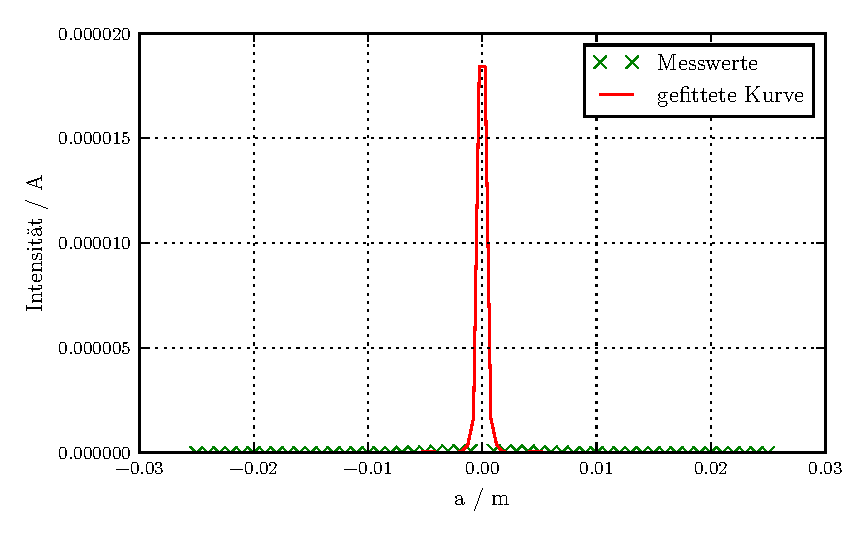
\includegraphics[height=9cm]{build/plot1.pdf}
  \caption{Ausgleichsrechnung zum dünnen Einzelspalt.}
  \label{fig:Einzel1}
\end{figure}

\begin{figure}[H] %Einzelspalt mittel
  \centering
  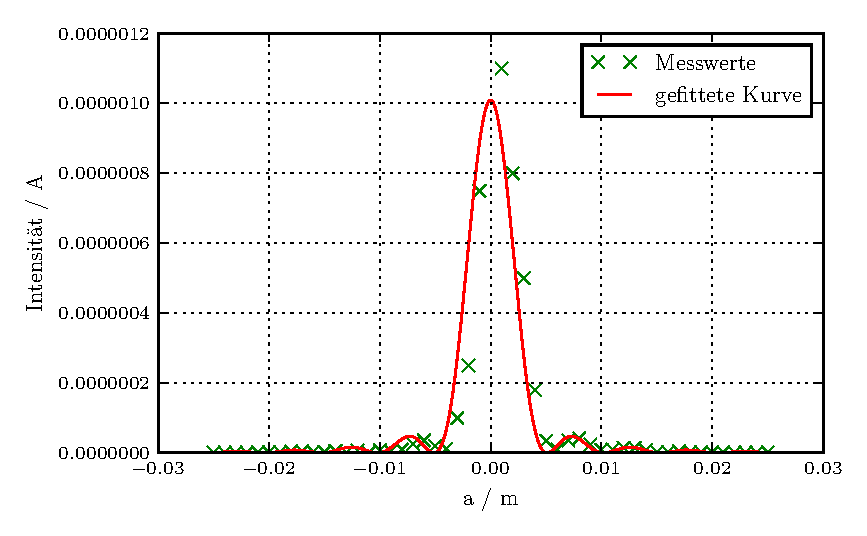
\includegraphics[height=9cm]{build/plot2.pdf}
  \caption{Ausgleichsrechnung zum mittleren Einzelspalt.}
  \label{fig:Einzel2}
\end{figure}

\begin{figure}[H] %Einzelspalt dick
  \centering
  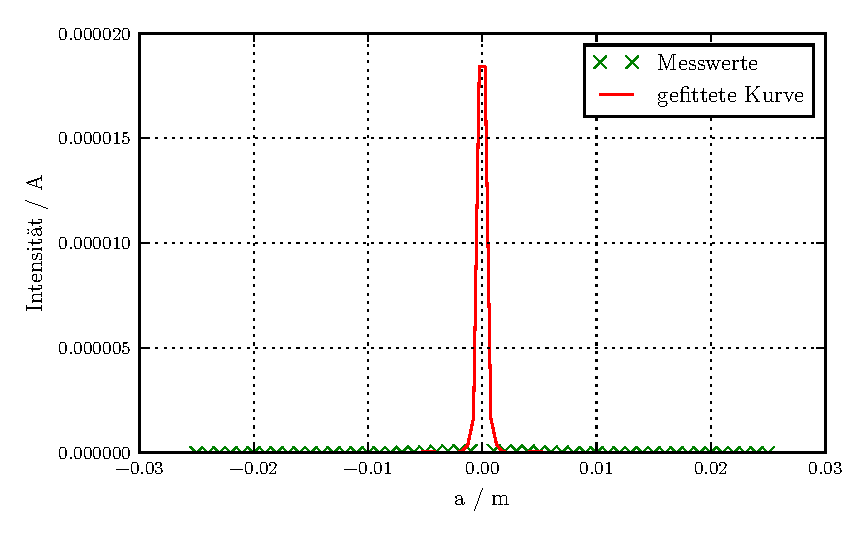
\includegraphics[height=9cm]{build/plot1.pdf}
  \caption{Ausgleichsrechnung zum dicken Einzelspalt.}
  \label{fig:Einzel3}
\end{figure}

\begin{figure}[H] %Doppelspalt
  \centering
  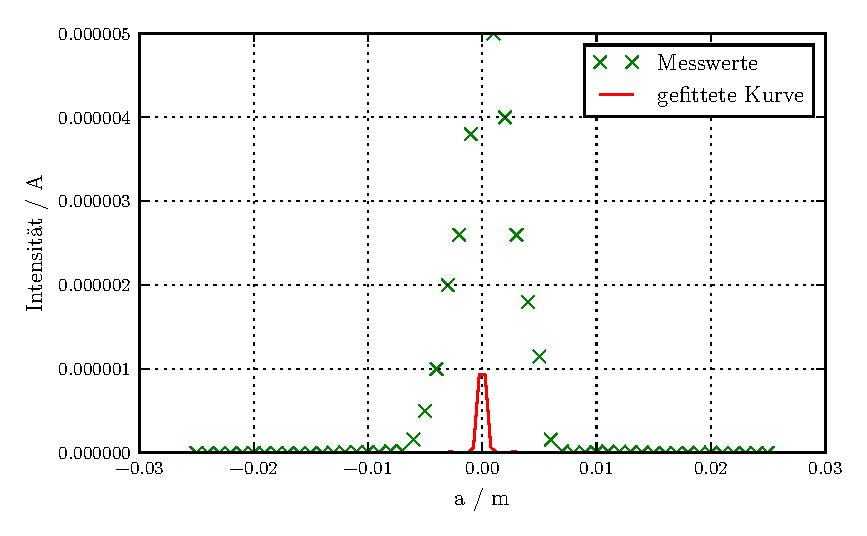
\includegraphics[height=9cm]{build/plot4.pdf}
  \caption{Ausgleichsrechnung zum Doppelspalt.}
  \label{fig:Doppel}
\end{figure}

Es ergeben sich folgende Werte für den dünnen Einzelspalt:
\begin{align*}
  \text{Spaltbreite per Intensitätsverteilung}:& \ b_\text{Beugung} = (\num{0.9999 +- 0.0}) \ \text{m} \\
  \text{Spaltbreite per Mikroskop}:& \ b_\text{Mikroskop} = 7.22 \cdot 10^{-5} \ \text{m} \\
  \text{Herstellerangabe}:& \ b_\text{Her} = 7.5 \cdot 10^{-5} \ \text{m} \\
  \text{Abweichung}:& \ \frac{b_\text{Her} \cdot 100}{b_\text{Beugung}} - 100 = 99.99 \% \\
  \text{Abweichung}:& \ \frac{b_\text{Mikroskop} \cdot 100}{b_\text{Beugung}} - 100 = 3.88 \%
\end{align*}

Es ergeben sich folgende Werte für den mittleren Einzelspalt:
\begin{align*}
  \text{Spaltbreite per Intensitätsverteilung}:& \ b_\text{Beugung} = (\num{1.0003 +- 0.0}) \ \text{m} \\
  \text{Spaltbreite per Mikroskop}:& \ b_\text{Mikroskop} = 1.33 \cdot 10^{-5} \ \text{m} \\
  \text{Herstellerangabe}:& \ b_\text{Her} = 1.5 \cdot 10^{-5} \ \text{m} \\
  \text{Abweichung}:& \ \frac{b_\text{Her} \cdot 100}{b_\text{Beugung}} - 100 = 99.99 \% \\
  \text{Abweichung}:& \ \frac{b_\text{Mikroskop} \cdot 100}{b_\text{Beugung}} - 100 = 12.78 \%
\end{align*}

Es ergeben sich folgende Werte für den dicken Einzelspalt:
\begin{align*}
  \text{Spaltbreite per Intensitätsverteilung}:& \ b_\text{Beugung} = (\num{0.9997 +- 0.0}) \ \text{m} \\
  \text{Spaltbreite per Mikroskop}:& \ b_\text{Mikroskop} = 4.0 \cdot 10^{-5} \ \text{m} \\
  \text{Herstellerangabe}:& \ b_\text{Her} = 4.0 \cdot 10^{-5} \ \text{m} \\
  \text{Abweichung}:& \ \frac{b_\text{Her} \cdot 100}{b_\text{Beugung}} - 100 = 99.96 \% \\
  \text{Abweichung}:& \ \frac{b_\text{Mikroskop} \cdot 100}{b_\text{Beugung}} - 100 = 0.00 \%
\end{align*}

Es ergeben sich folgende Werte für den Doppelspalt:
\begin{align*}
  \text{Spaltbreite}:& \ b_\text{Beugung} = (\num{1.0018 +- 0.0}) \ \text{m} \\
  \text{Spaltabstand}:& \ s_\text{Beugung} = (\num{0.9968 +- 0.0}) \ \text{m} \\
  \text{Herstellerangabe}:& \ b_\text{Her} = 1.0 \cdot 10^{-5} \ \text{m} \\
  \text{Herstellerangabe}:& \ s_\text{Her} = 4.0 \cdot 10^{-5} \ \text{m} \\
  \text{Abweichung}:& \ \frac{b_\text{Her} \cdot 100}{b_\text{Beugung}} - 100 = 99.99 \% \\
    \text{Abweichung}:& \ \frac{s_\text{Her} \cdot 100}{s_\text{Beugung}} - 100 = 99.96 \% \\
\end{align*}
